\documentclass[a4paper,10pt]{article}

\usepackage[polish]{babel}
\usepackage[utf8]{inputenc}
\usepackage[OT4]{fontenc}
\usepackage{float}
\usepackage{abstract}
\usepackage{graphicx}
\usepackage{standalone}

\usepackage{pgfplots}
\usepackage{tikz}
\usetikzlibrary{shapes,arrows,arrows.meta}
\pgfplotsset{compat=1.13}
\usepackage{mathtools}
\usepackage{amssymb}

\bibliographystyle{plplain} % styl bibliografii (plplain -- z językiem polskim)
\date{23 stycznia 2020}

\newcommand{\album}[1]{\unskip ,~#1}

\title{Wizualizacja zdalnie zarządzanego termostatu}
\author{Dawid Sienkiewicz \album{35918} }
\begin{document}

\maketitle\mbox{}\\\\\\
\begin{abstract}
Celem tej pracy jest stworzenie zarządzanego zdalnie poprzez smartfona termostatu \cite{ThermostatWiki}.

Termostat to urządzenie utrzymujące zadaną temperaturę. Sprawa jest dość prosta, gdy mamy fizyczny dostęp do takiego urządzenia i w zależności od potrzeb, możemy nim sterować. Co jednak, gdy nasze mieszkanie, dom lub inny obiekt odległy jest w wiele kilometrów, wyjeżdżamy na wakacje, a chcemy podtrzymywać temperaturę w jakimś pomieszczeniu i mieć nad tym ciąglą konktrolę. Ze względów praktycznych (załącznie przed przyjazdem, informacja o aktualnych warunkach) i bezpieczeństwa (alerty bezpieczeństwa). Odpowiedzią na takie wymagania ma być ten projekt.

\end{abstract}
\newpage
\tableofcontents
\newpage
\section{Podstawowe wymagania biznesowe}
\label{zalozenia_projektu}

Przy określaniu technologii powinniśmy brać pod uwagę przede wszystkim optykę użytkownika końcowego. Główne założenia przedstawione zostały poniżej:\\ 

\begin{itemize}
    \item Prosta obsługa termostatu
	\item Duża dostępność do urządzenia niezależnie od odległości
    \item Wieloplatformowość zastosowanych rozwiązań
	\item Interfejs użytkownika powinien działać na popularnym sprzęcie dostępnym dla więkoszści użytkowników
	\item Łatwy dostęp do platformy sprzętowej, opartej na masowej produkcji
	\item Niski koszt jednostkowy całego rozwiązania
\end{itemize}

\section{Opis urządzenia}
\label{opis_systemu}
Termostat posiada funkcję zdalnego dostępu poprzez usługę w chmurze. Użyto w tym celu autorskiej platformy ELTRA \cite{EltraWebsite}. \\

Urządzenie pozwala na:

\begin{itemize}
    \item Odczyt stanu urządzenia
    \item Odczyt podstawowych parametrów (temperatura, wilgotność, ciśnienie)
    \item Odczyt i prezentacja historii zmian
    \item Wyświetlanie statystyk
    \item Parametryzowanie nastawów termostatu
\end{itemize}

\section{Architektura systemu}
\label{architektura_systemu}

Jego ogólną architekturę przedstawia Rysunek \ref{rysunek_architektura_systemu}. Architektura opiera się na klasycznym modelu gwiazdy w którym punktem centralnym jest usługa w internecie. Urządzenie nadzorcze kontaktuje się z usługą w chmurze \cite{CloudExplained}, aby po uzyskaniu autoryzacji móc wymieniać komunikaty z udostępnionym urządzeniem sterującym. Urządzenie nadzorcze (master), także wymienia komunikaty z usługą w chmurze. Komunikacja odbywa się wyłącznie z udziałem tej usługi sieciowej. \\

System składa się z trzech podstawowych elementów:

\begin{itemize}
    \item Usługi sieciowej w chmurze (ELTRA \cite{EltraWebsite})
    \item Urządzenia sterujacego (Raspberry Pi\cite{RaspberryPiWiki})
    \item Urządzenia nadzorczego i prezentującego dane (smartfon Android\cite{AndroidWiki}, iOS\cite{IOSWiki})
\end{itemize}

Zastosowanie i uzasadnienie wyboru poszczególnych elementów zostanie opisane niżej.

\begin{figure}[H]
\begin{center}
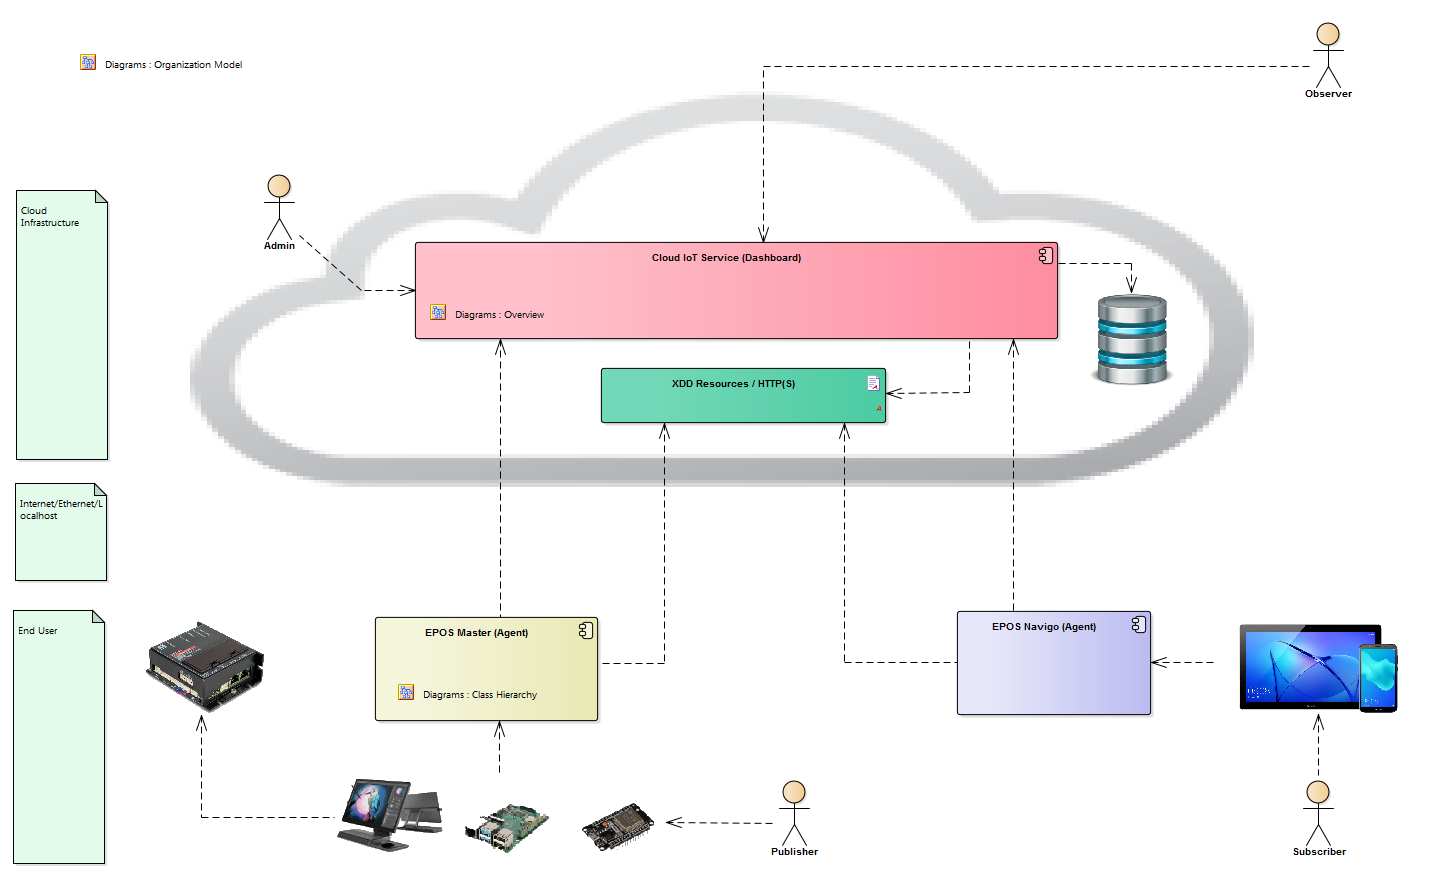
\includegraphics[width=1.0\textwidth]{eltra.png}
\end{center}
\caption{Platforma ELTRA - Ogólna architektura systemu}
\label{rysunek_architektura_systemu}
\end{figure}

\section{Usługa sieciowa}
\label{usluga_sieciowa}

Usługa sieciowa bazuje na serwerze VPS (Virtual Private Server)\cite{VPSWiki} dostępnym pod publicznym adresem IP oraz działającym na nim serwerze WWW \cite{WWWWiki} oraz bazy danych SQL \cite{MySQLWiki}.\\

Serwer WWW wspiera następujące technologie służące do wymiany danych:

\begin{itemize}
    \item RESTful API - klasyczny interfejs używny w serwisach www \cite{RestApiWiki}
    \item Protokół WebSocket \cite{WebsocketWiki} - dwukierunkowa komunikacja poprzez TCP/IP
\end{itemize}

Wybór konkretnie tych technologii nie był przypadkowy. Chodziło z jednej strony o zastosowanie standardowego w świecie usług sieciowych API jak REST dla zapewnienia szerokiego wsparcia ze strony praktycznie dowolnej technologii programistycznej. Technologia Websocket \cite{WebsocketWiki} z kolei pozwala na rozszerzenie funkcjonalności serwisu o asynchorniczną i pozbawioną konieczności częstego odpytywania funkcjonalność.

\section{Urządzenie sterujące}
\label{urzadzenie_sterujace}

Urządzenie sterujące jest w praktyce mini-komputerem (komputerem o niewielkich rozmiarach pokroju karty kredytowej), które posiada wejścia cyfrowe i/lub analogowe pozwalające podłączyć zewnętrzne urządzenia takie jak sensory, czy sterowniki.\\
W praktyce takie urządznie ma być możliwe tanie, potrafić komunikować się z sewerem sieciowym oraz podłączonymi urządzeniami. \\\\\\

Wybrane sprzętowe komponenty systemu:
\begin{itemize}
    \item Minikomputer Raspberry PI 3 \cite{RpiWiki}
    \item Sensor temperatury i wilgotności DHT11 
    \item Sensor temperatury BMP180 (dodatkowy sensor do pomiaru temperatury zewnętrznej)
    \item Cyfrowy przekaźnik 230V (sterowanie grzejnikiem)
\end{itemize}

Zastosowanie Raspberry PI podyktowane jest bezproblemową dostępnością tej platformy sprzętowej, relatywnie niską ceną urządzenia (ok. 120 zł) i możliwością użycia na nim systemu operacyjnego Linux.\\

Sensory DHT11 i BMP180 to niskokosztowe sensory używające sygnału cyfrowego dostępnego standardowo na Raspberry PI poprzez wejścia GPIO (general purpose input output) oraz I2C\cite{I2CWiki} przez co nie wymagają dodatkowego sprzętu. 

Po poprawnej konfiguracji sprzętowej nasz system może odczytywać dane z podłączonych sensorów. 

\paragraph{Krótki opis działania} 
Odpowiednie  oprogramowanie komunikuje się w regularnych odstępach czasu z sensorami i dokonuje odczytów. W zależności do ustawionych progów, program poprzez przekaźnik automatycznie steruje grzejnikiem. W tym samym czasie komunikuje się z serwerem sieciowym przekazując dane o swoim stanie, odczytach z sensorów oraz pozwala na manipulacje ustawień systemu, takimi jak progi temperatury, załącznie i wyłączenie całego urządzenia, etc.

\paragraph{Uśrednianie wyników} W trakcie pracy sensory mogą otrzymywać błędne odczyty poza skalą poprawnych wyników. Dla usunięcia tych błędów oraz wygładzenia przebiegu funkcji wzrostów i spadków danych pomiarowych zastosowano tzw. Filtr Kalmana \cite{KalmanWiki}, który przedstawia rysunek \ref{diagram_kalman}

\begin{figure}[H]
\label{diagram_kalman}
\centering
\begin{minipage}{1\textwidth}
\centering
\documentclass[varwidth=true, border=2pt]{standalone}

\usepackage{pgfplots}
\usepackage{tikz}
\usetikzlibrary{shapes,arrows,arrows.meta}
\pgfplotsset{compat=1.13}
\usepackage{mathtools}
\usepackage{amssymb}

\begin{document}
\tikzstyle{block} = [draw, rectangle, minimum width=6em, align=center,fill=gray!5]
\tikzstyle{arrow} = [-latex, very thick]
\newcommand*{\tran}{\top}

\begin{tikzpicture}[auto, node distance=2cm,>=latex']
    \setlength{\abovedisplayskip}{0pt}

    % Place the blocks
    \node[text width=1cm,
          rounded corners=3pt,
          block,
          label={[above,align=center]{Initial\\State}}] at (-1, 0) (initial)
          {$$\mathbf{x}_0$$  $$P_0$$};
    \node at (0.25, 0.1) (sum) {};
    \node[block, text width=6cm,
          label={[above,align=center]{Prediction}}] at (4, 0) (prediction)
          {\begin{align*}
            \mathbf{x}_{k+1}^{(P)} &= A \mathbf{x}_k + B {\color{orange} a_k}\\
            P_{k+1}^{(P)} &= A P_k A^\tran + C_k^{(r_s)}
           \end{align*}};
    \node [block, right of=prediction,
            node distance=3cm, text width=1.4cm] at (6, -2) (iterUpdate)
            {$$k \leftarrow k + 1$$};
    \node [block, text width=6cm,
           label={[above,align=center]{Innovation}}] at (4, -4) (innovation)
           {\begin{align*}
              K_k &= P_k^{(P)} H^\tran {\left (H P_k^{(P)} H^\tran + C_k^{(r_m)} \right)}^{-1}\\
              {\color{blue} \mathbf{x}_k} &= (I - K_k H) \mathbf{x}_k^{(P)} + K_k {\color{orange} z_k}\\
              {\color{blue} P_k} &= (I - K_k H) P_k^{(P)}
            \end{align*}};

    % Connect the nodes
    \draw [arrow] (initial) -- (prediction);
    \draw [arrow] (prediction.east) -| (iterUpdate.north);
    \draw [arrow] (iterUpdate) |- (innovation);
    \draw [arrow] (innovation.west) -|  (sum);
\end{tikzpicture}

\end{document}

\end{minipage}
\caption{Filtr Kalman'a}
\end{figure}

\section{Interfejs użytkownika}

\subsection{Urządzenie nadzorujące}
\label{interfejs_uzytkownika}
Jednym z głównych założeniem projektu, była duża elastyczność w doborze metody prezentowania danych.
Zastosowanie REST API\cite{RestApiWiki} pozwala na implementacje takiego interfejsu użytkownika w wielu językach i technologiach. 
Interfejs powinien być dostępny na popularnych urządzeniach przenośnych typu smartfon lub tablet, stacjonarnych komputerach z systemem Windows 10 i docelowo pod dowolnym systemem z obsługą stron WWW.\\

Wspierane przez interfejs użytkownika platformy:
\begin{itemize}
    \item Android (Google) \cite{GoogleWiki}
    \item Windows 10 (Microsoft) \cite{Windows10Wiki}
	\item iOS (Apple) \cite{IOSWiki}
	\item Inne platformy poprzez przeglądarkę WWW
\end{itemize}

W tym projekcie przyjęto do rozwiązanie zaproponowane przez firmę Microsoft\cite{MicrosoftWiki} i jej multiplatformowe narzędzie o nazwie Xamarin\cite{XamarinWiki}. Zaletą tego podejścia jest nie tylko używanie jednej technologii jaką jest .NET\cite{DotNetWiki} firmy Microsoft, ale też używanie wspólnego kodu źródłowego w języku C\# \cite{CSharpWiki} do implementacji całej aplikacji.

\subsection{Podgląd stanu i zarządzanie termostatem}

Do podglądu stanu termostatu używany jest program w ELTRA Navigo\cite{EltraNavigoGooglePlay}, który korzysta z technologii wspomnianych w podrozdziale  \ref{interfejs_uzytkownika}.\\
Aplikacja Navigo zwalnia nas z potrzeby troszczenia się o wymianę danych z termostatem. Proces inicjalizacji urządzenia sprowadza się w skrócie do:

\begin{enumerate}
    \item Połączenie z usługą w chmurze
    \item Podania danych autoryzacyjnych zdalnego urządzenia
    \item Pobrania danych samego urządzenia (wersja, położenie)
    \item Pobrania wspieranych usług urządzenia \cite{FDTWiki}
    \item Pobrania wspieranych objektów \cite{CANOpenDictWiki}
    \item Obsługiwanego interfejsu użytkownika (wspierane UI)
\end{enumerate}

Po poprawnej autoryzacji otrzymujemy możliwość poprzez panele 'Overview' i 'Control' podglądu stanu i zarządzania urządzeniem poprzez np. ustawianie minimalnej i maksymalnej temperatury pracy, tak jak pokazane jest na Rysunkach \ref{rysunek_navigo_overview} i \ref{rysunek_navigo_control}\\
Warto wspomnieć, że sama koncepcja pobierania usług wspieranych przez urządzanie jest oparta o standard FDT\cite{FDTWiki}, szeroko stosowaną w automatyce.

\begin{figure}[H]
    \centering
    \begin{minipage}{0.45\textwidth}
        \centering
        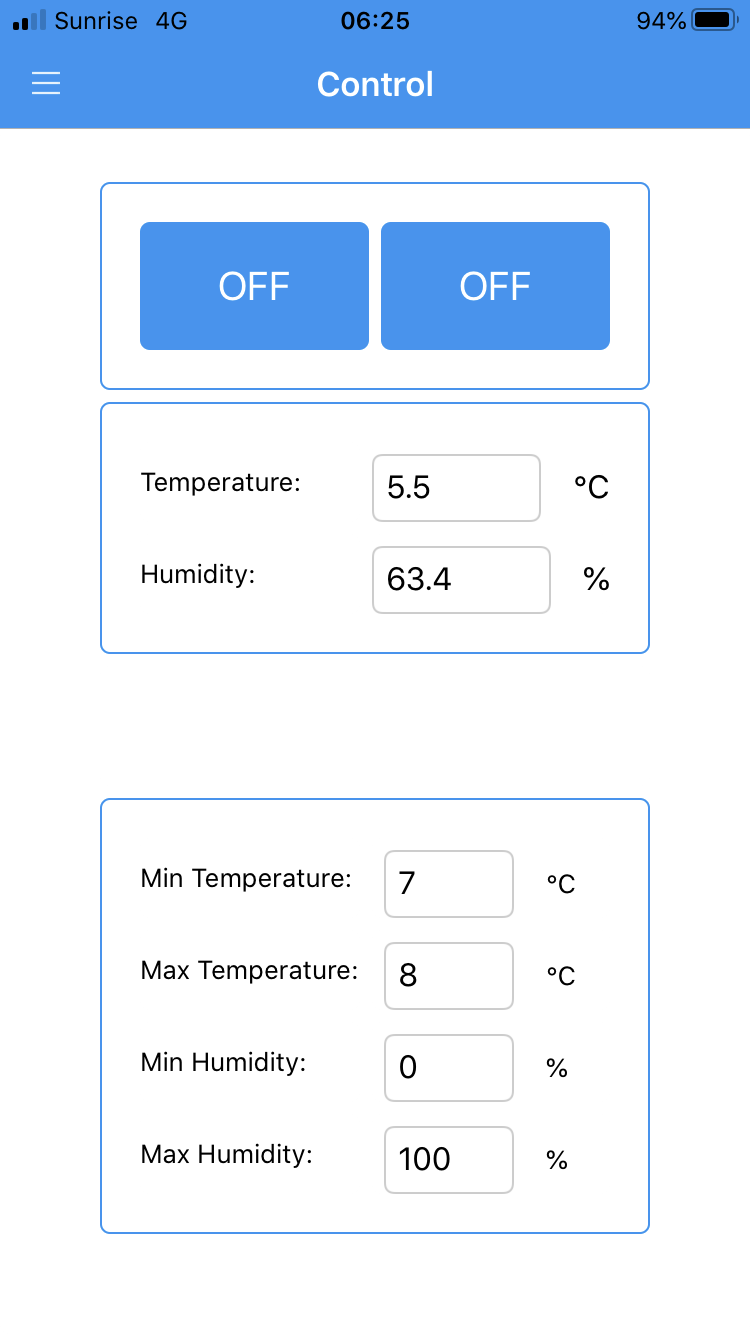
\includegraphics[width=0.9\textwidth]{navigo_control.png} 
        \caption{ELTRA Navigo - Kontrola nastawów termostatu}
        \label{rysunek_navigo_control}
    \end{minipage}\hfill
    \begin{minipage}{0.45\textwidth}
        \centering
        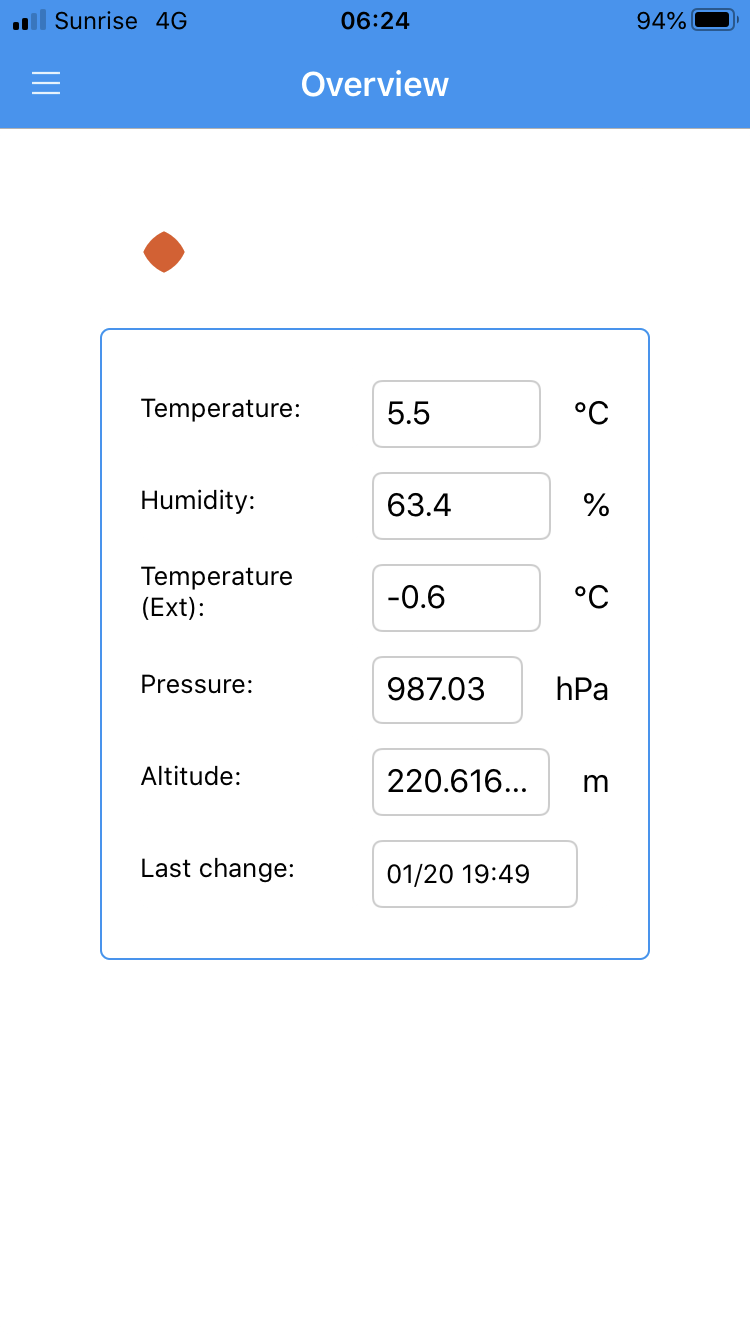
\includegraphics[width=0.9\textwidth]{navigo_overview.png}
        \caption{ELTRA Navigo - Podgląd stanu}
        \label{rysunek_navigo_overview}
    \end{minipage}
\end{figure}

\subsection{Podgląd historii zmian parametrów}

Jedną z interesujących funkcji platformy ELTRA\cite{EltraWebsite} jest możliwość pobierania historii zmian dowolnego parametru w zdefiniowanym przedziale czasu. Może to być używane do prezentacji historii przebiegów parametrów podstawowych, takich jak temperatura, czy wilgotność, ale także do prowadzenia statystyk załączeń grzejnika. Dysponując informacjami historycznymi możemy nie tylko wyświetlić interesujące wykresy, ale także obliczyć koszt pracy urządzania (znając ilość załączeń). 

\begin{figure}[H]
    \centering
    \begin{minipage}{0.45\textwidth}
        \centering
        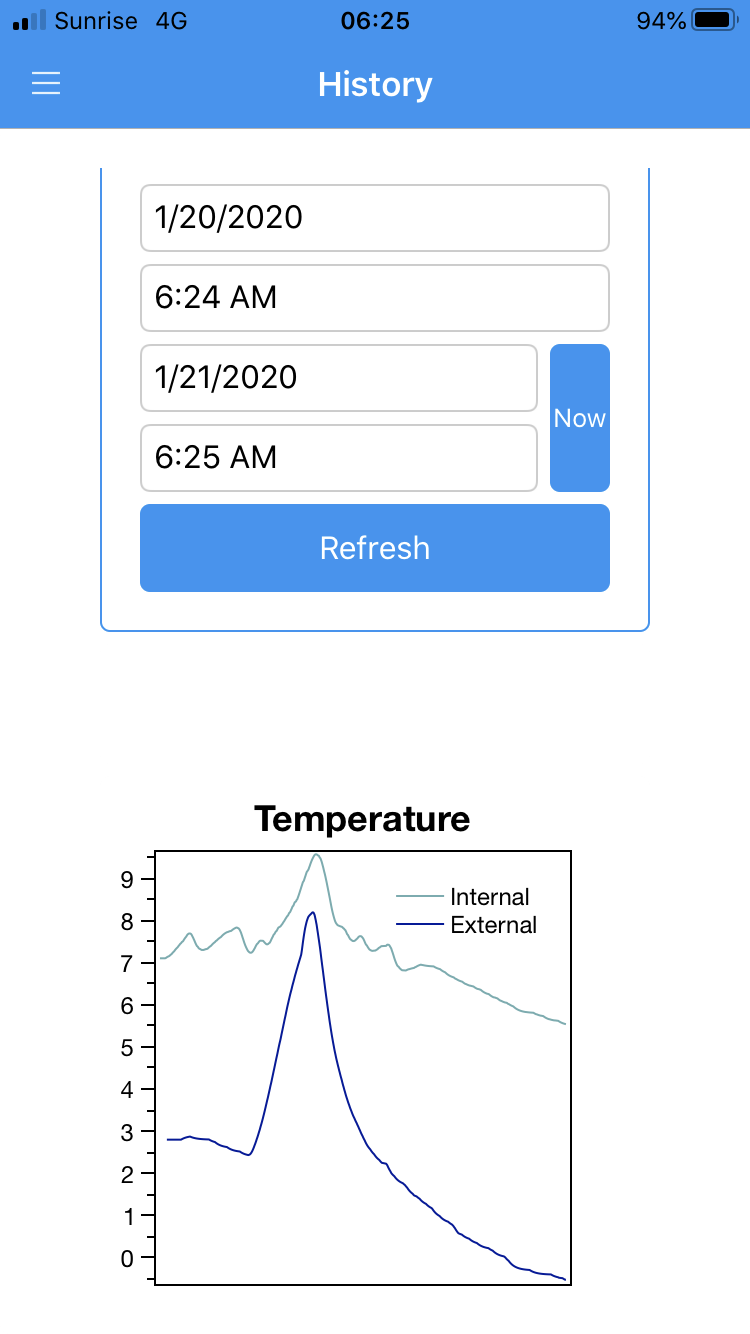
\includegraphics[width=0.9\textwidth]{navigo_history1.png} % first figure itself
        \caption{ELTRA Navigo - Historia zmian / temperatura}
        \label{rysunek_navigo_history_1}
    \end{minipage}\hfill
    \begin{minipage}{0.45\textwidth}
        \centering
        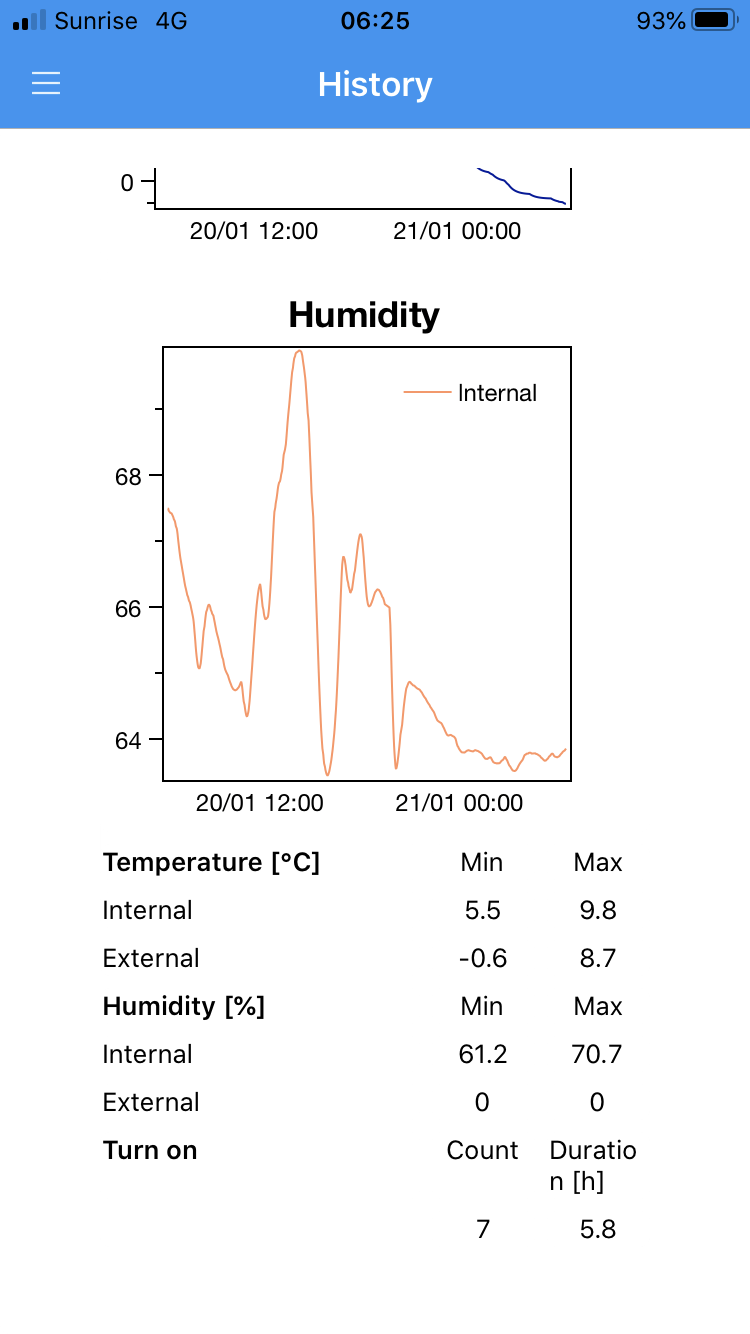
\includegraphics[width=0.9\textwidth]{navigo_history2.png} % second figure itself
        \caption{ELTRA Navigo - Historia zmian / wilgotność}
        \label{rysunek_navigo_history_2}
    \end{minipage}
\end{figure}

\section{Podsumowanie}

Projekt termostatu wydaje się być prostym zagadnieniem. Celem projektu było jednak stworzenie uniwersalnego i łatwego do rozszerzeń rozwiązania. W trakcie realizacji pojawiło się wiele złożonych zagadnień, które same w sobie nie są trywialne.

\begin{enumerate}
    \item Komunikacja hybrydowa RESTful/WebSocket
    \item Protokoły wykorzystywane w automatyce, takie jak CANOpen\cite{CANOpenDictWiki}, czy FDT\cite{FDTWiki}
    \item Obsługi komunikacji z sensorami poprzez interfejsy I2C\cite{I2CWiki}, czy GPIO
    \item Używanie zaawansowanych algorytmów matematycznych, takich jak filtr Kalmana\cite{KalmanWiki}
    \item Implementacja interfejsu przy użyciu multiplatformowego frameworku Xamarin\cite{XamarinWiki}
\end{enumerate}

Powstałe rozwiązanie jest też na tyle uniwersalne, że dostosowanie, go do innych wymagań lub zastosowań staje się bardzo proste. Sprowadza się w praktyce do zdefiniowania własnych obiektów. Implementacji ustawiania tych obiektów po stronie urządzenia sterującego i wyświetlania po stronie aplikacji nadzorującej. 

\bibliography{biblio}

\end{document}